\chapter{Test of Vanna-Volga Pricing}


\section{Data Source}
\subsection{Volatility Matrix}
Volatity matrix data in terms of ATM, $10\Delta$, and 25$\Delta$ butterflies (BF) and risk reversals (RR) of FX derivatives for Vanna-Volga models was sourced from Bloomberg. An example of volatility matrix data of EUR/USD observed on May 10, 2017 with 1M maturity was showing below.

\begin{figure}[htb]
	\centering
	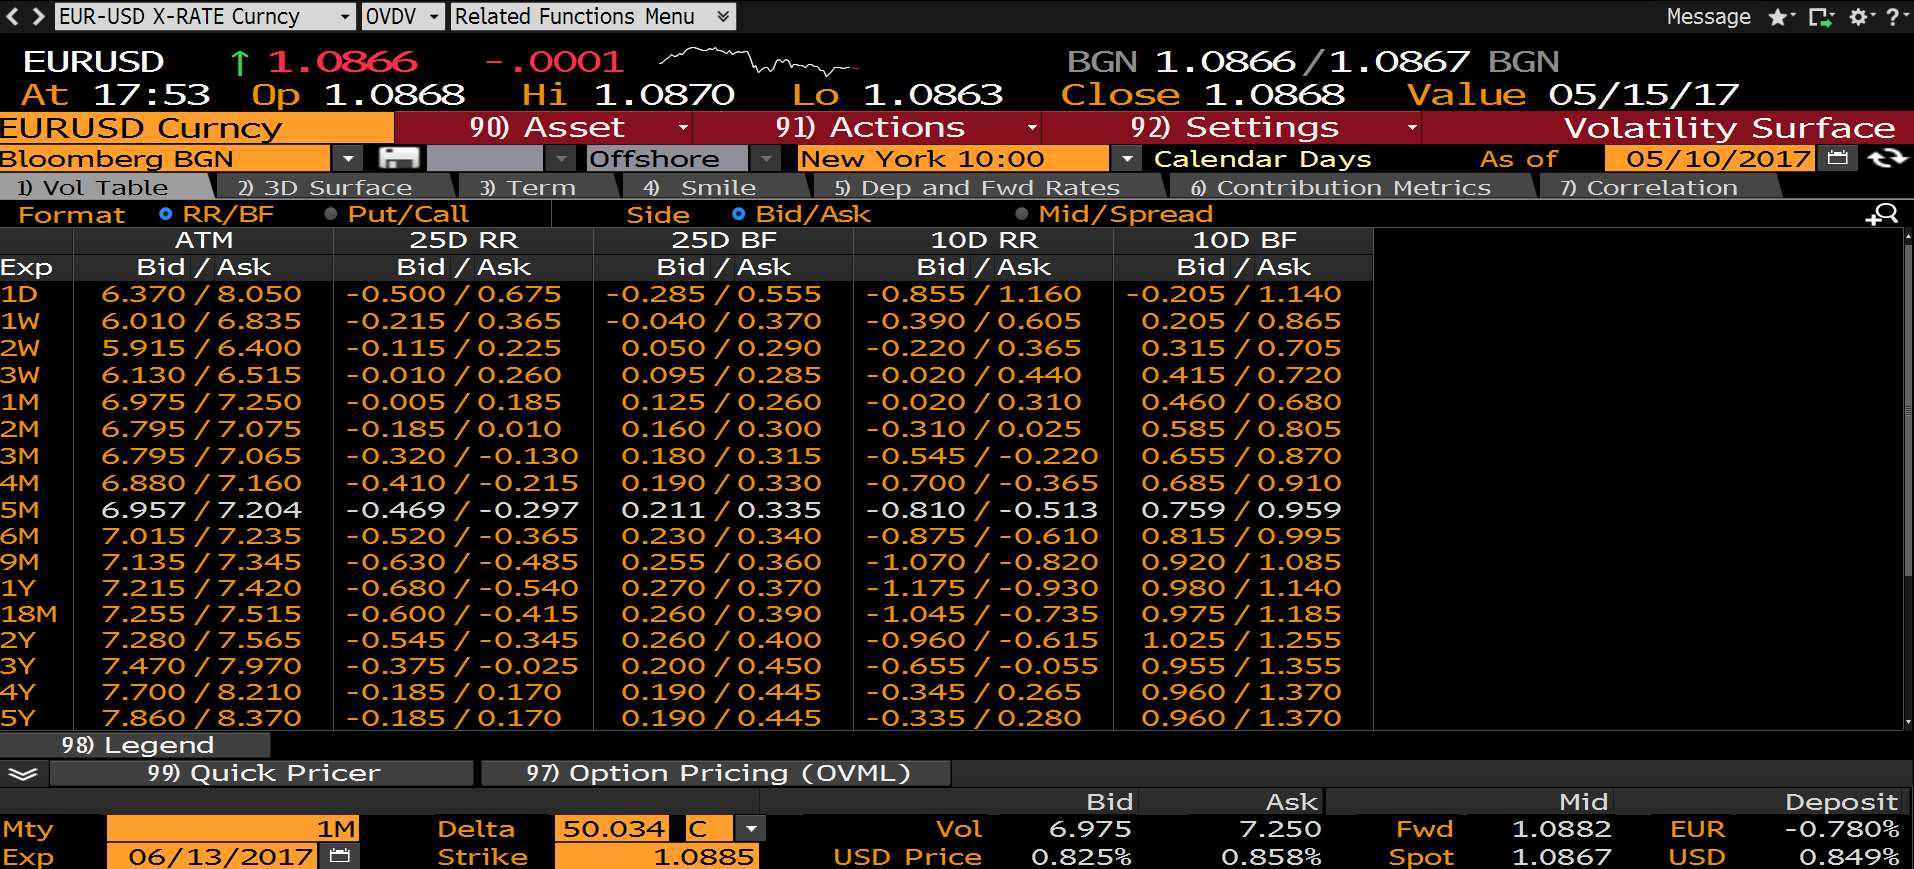
\includegraphics[scale=0.3]{./Testing-data/VolMatrix/EURUSD_1M_vol.png} 
	\caption{Volatility matrix data in the bid/ask format in terms of ATM, $10\Delta$, and $25\Delta$ butterflies (BF) and risk reversals (RR), observed on May 10, 2017. Source: \textit{Bloomberg}}
	\label{fig:label} % insert suitable label, this is used to refer to a fig from within the text as shown above
\end{figure}
\noindent
In order to verify the price calculated by using Vanna-Volga model, two benchmark prices (Heston model from Bloomberg pricing tools and \textit{investing.com} with price provided by \textit{Sentry Derivatives}) for FX derivatives had been put in \textit{Appendix A.3}. Since Vanna-Volga is an analytically derived correction to Black-Scholes model, the price calucluated by Black-Scholes model also had been included for analysis.
\newline
\newline
The interest rates used for Vanna-Volga model and Black-Scholes model were obtained from \textit{www.tradingeconomics.com} and listed in the following table.

\begin{table}[htb]
\centering
\caption{{FX interest rates observed on May 10, 2017}}
\begin{tabular}{ccc}
\hline	\hline % insert double horizontal line
Symbol & USD & EUR   \\ [1ex]% heading
\hline
Rates & 1.00\% & 0.00\%    \\ [1ex]
\hline
\end{tabular}
\label{table:FX_rates}
\end{table}

\subsection{Model Implementation}
As the volatility matrix obtianed from Bloomberg is in the bid/ask format, the averaged mid volatility was used for Black-Scholes model and Vanna-Volga model. The mid volatility matrix data of FX derivatives were list below. And we consider that live exchange rate as the initial price of FX options $S_0$.
\newline
\newline
Since Vanna-Volga model is limited to the short-dated (tipically less than 1Y) FX options, a test of EUR/USD call options with 1Y maturity also had been conducted with same procedure of 1M maturity.
\begin{table}[htb]
\centering
\caption{Mid volatility matrix of EUR/USD with 1M maturity}
\begin{tabular}{ccccccc}
\hline \hline
FX derivatives & ATM  & 25D RR  & 25D BF  & 10D RR  & 10D BF & $S_0$\\ [0.5ex]
\hline 
EUR/USD  & 7.1125 &0.09& 0.1925 &0.145 &0.57&1.0866 \\[0.5ex]
\hline
\end{tabular}
\end{table}

\begin{table}[htb]
	\centering
	\caption{Mid volatility matrix of EUR/USD with 1Y maturity}
	\begin{tabular}{ccccccc}
		\hline \hline
		FX derivatives & ATM  & 25D RR  & 25D BF  & 10D RR  & 10D BF & $S_0$\\ [0.5ex]
		\hline 
		EUR/USD  & 7.415&	-0.685&	0.325&	-1.175	&1.065 &1.0923\\[0.5ex]
		\hline
	\end{tabular}
\end{table}

\noindent
With the conventions and definitions specified in \textbf{Technical Specification}, the implementation of Black-Scholes model and Vanna-Volga model of FX derivatives had been coded in jupyter notebook with Python 3.5 in \textit{Appendix A.3}.

\section{Testing Results}
In order to compare the prices calculated from Vanna-Volga to the benchmark prices easily, we define the price to be \% FOR (foreign currency). For example, we use \% EUR to be the price form of Vanna-Volga model for EUR/USD options.
\subsection{Short-dated Maturity}
The results from the implemented codes with EUR/USD call option had been put in the table. The details of the prices of four methods corresponding to the strike could be found in \textit{Appendix A.3}.

\begin{table}[htb]
\centering
\caption{Prices of EUR/USD call option with 1M matiruty}
\begin{tabular}{ccccc}
\hline \hline
Strike & Heston & investing.com & BS & Vanna-Volga \\ [0.5ex]
\hline
1.065 &	0.023241&	0.0233	&0.024682&	0.023363 \\ 
1.070&	0.019381&	0.0195&	0.020663&	0.019671\\
1.075	&0.015802&	0.0160&	0.016970&	0.016277 \\
1.080	&0.012571&	0.0128&	0.013649&	0.013224\\
1.085	&0.009770&	0.0101&	0.010733&	0.010544 \\ [0.5ex]
\hline
\end{tabular}
\label{table:prices-1M}
\end{table}

\noindent
From the table, we could find that the prices of Vanna-Volga were close to the prices of Bloomberg and investing.com. In particular, Vanna-Volga prices were very close to the prices used in investing.com. In order to visualize the results, a figure contained all the prices had been put in the below.

\begin{figure}[htb]
	\centering
\includegraphics[scale=0.4]{./Testing-data/Python-codes/Python-4prices-1M.png} 
\caption{Prices of EUR/USD call options with 1M maturity. Data observed on May 10, 2017}
\label{fig:prices-label} % insert suitable label, this is used to refer to a fig from within the text as shown above
\end{figure}

\noindent
The figure clearly showed that the prices calculated through Vanna-Volga model were very close to the benchmark prices. Besides, as we might see, the Black-Scholes prices (green line) were far away from the benchmark prices compared to Vanna-Volga prices. This figure was consistent with the purpose of the Vanna-Volga model, which is that Vanna-Volga model is an analytically derived correction by capturing the greeks of vanna and volga to Black-Scholes model.

\subsection{1Y Maturity}

Following the same procedure, we got the result as following.

\begin{table}[htb]
	\centering
	\caption{Prices of EUR/USD call option with 1Y matiruty}
	\begin{tabular}{ccccc}
		\hline \hline
		Strike & Heston & investing.com & BS & Vanna-Volga \\ [0.5ex]
		\hline
		1.05 &	0.069127&	0.0695&	0.065060&	0.058870 \\ 
		1.06&	0.062125&	0.0623	&0.058001&	0.052372\\
		1.07&	0.055455&	0.0555&	0.051381&	0.046276 \\
		1.08&	0.049155&	0.0490	&0.045220&	0.040596\\
		1.09&	0.043257&	0.0429	&0.039532&	0.035339 \\ [0.5ex]
		\hline
	\end{tabular}
	\label{table:prices-1Y}
\end{table}
\noindent
From the table, we found that two benchmark prices (Heston from Bloomberg pricing tools and prices from \textit{investing.com}) are very close. However, Black-Scholes prices were much far away from the benchmark prices and the Vanna-Volga prices were even far away from the benchmark prices. In order to visualize the results, a figure contained all the prices had been put in the below.

\begin{figure}[htb]
	\centering
	\includegraphics[scale=0.4]{./Testing-data/Python-codes/Python-4prices-1Y.png} 
	\caption{Prices of EUR/USD call options with 1Y maturity. Data observed on May 12, 2017}
	\label{fig:prices-1Y-MAY12} % insert suitable label, this is used to refer to a fig from within the text as shown above
\end{figure}
\noindent
The figure clearly showed that both Black-Scholes prices and Vanna-Volga prices were far away from the benchmark prices, which implied that the Black-Scholes model and Vanna-Volga model were not good for long-dated maturity FX options.

\subsection{Test Conclusion}
\noindent
Therefore, we conclued that the model is valid and appropriate for short-dated (less than 1Y) maturity FX vanilla options pricing, which was the conditions of using Vanna-Volga models. In summary, the Vanna-Volga model is good for pricing FX options. As the limitation of the report, only FX vanilla options pricing had been tested. However, Agnieszka Janek showed that Vanna-Volga model was also good for pricing first-generation FX options, e.g., FX barrier options. His paper had been included in the references list.

